\chapter{The Graph Neural Network Model}

In this chapter we introduce our Graph Neural Network model and discuss related literature that use neural networks for classification problems on graph structured data. 

\section{Graph Neural Network}

The Graph Neural Network (GNN) is a flexible neural network architecture that is based on two local operators on a graph $G = (V, E)$. Given some $l$-dimensional input signal $F :V \rightarrow \mathbb{R}^{n \times l}$ on the vertices $V$ of an $n$-vertex graph $G$ (we call such a function a $l$-dimensional signal on graph $G$, where $l$ is arbitrary), we consider two operators that act locally on this signal as well as a non-linearity operator.\\

\begin{definition}Define the \textit{degree operator} as a map $D : F \mapsto D(F)$ where $$(D(F))_i := deg(i) \cdot F_i$$  where $deg(i)$ is the degree of vertex $i \in V$.  
\end{definition}
\begin{definition}Define the \textit{adjacency operator} as a map $W: F \mapsto W(F)$ where $$(W(F))_i:= \sum_{j\sim i }F_j$$ where $i \sim j$ means vertex $i$ is adjacent to vertex $j$. 
\end{definition}

\begin{definition}Define the \textit{pointwise nonlinearity operator} as a map $\eta_{\theta}: \mathbb{R}^p \cdot \mathbb{R}^p \rightarrow \mathbb{R}^q$ parametrized by some $\theta \in \mathbb{R}^l$ trainable. An example of such an operator is the convolution operator used in convolutional neural networks.\\
\end{definition}

\begin{figure}
\begin{center}
  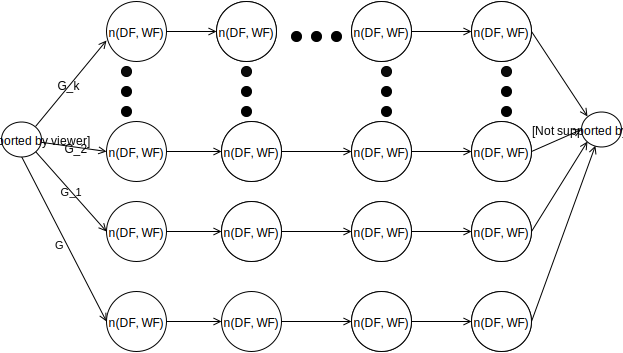
\includegraphics[width=\textwidth]{GNN.png}
  \caption{An example of an architecture constructed from operators D, W and $\theta$}
  \label{fig:GNN}
 \end{center}
\end{figure}

One layer of applying $D$ and $W$ allows us to recover the graph Laplacian operator.  To be precise, let $F$ be a $p$-dimensional signal on $G$ , then if we define $$ \eta(DF, WF) := DF - WF$$ we can recover the unnormalized graph Laplacian.  If we further define operators $D^{-1/2}$ and $D^{-1}$ (which will be analogously defined to the degree operator $D$, only with entries multiplied by the entriees of $D^{-1/2}$ and $D^{-1}$ instead of that of $D$), we will similarly be able to recover the symmetric and random walk Laplacians.  Furthermore, by stacking together several of the Laplacian operators above, and allowing ourselves to renormalize the signal after each application, we are able to recreate the power method. This is because we are simply applying the Laplacian operator many times while renormalizing before each application. Therefore the expressive power of this GNN includes approximations to eigendecompositions.\\

\subsection{Related Work}
The GNN was first proposed in \cite{GNN} as a way to approximate signals on graphs. Bruna et al. also generalized convolutions for signals on graphs in \cite{Bruna}.  Their idea was that the convolution neural network architecture, so successful for image data, can be interpreted as learning to representing image signals in the very rapidly decaying Fourier basis.  The coefficients of representing the signals in this basis is rapidly decaying because images lie on very regular graphs (in particular grids). This generalization of the convolution allowed them to use the graph Laplacian's eigenbasis to create a general graph convolution.  The authors successfully applied this neural network for signals on meshes.  Kipf and Welling showed more recently in \cite{kipf2016semi} the GNN with only two symmetric Laplacian layers, can be quite effective as a embedding procedure for graph signals.  They applied their network to semi-supervised learning problems where some graph nodes were labelled but others were not.\\

The present work is the first time a neural network has been applied to community detection.  Furthermore because we are applying it to SBMs at the information theoretic threshold, the graphs we are dealing with are far sparser then all previous applications.   We are able to show that our version of the GNN can compete with algorithms doing  clustering on the SBM in even the hardest of regimes (detectability).  This will not work with previous GNN architectures mentioned above.  In addition, we are not doing an eigendecomposition, which is required of spectral algorithms, thus making the network more efficient computationally.  %Lastly we apply the GNN to extremely large graphs, with millions of nodes.  These real datasets have ground truth communities which we compare the performance of.  



